\subsection{Chapter 5 - Newton's Laws}

\subsubsection{Overview}\label{chap:NewtonsLaws}

In this chapter, we introduce Newton's Laws, which is a succinct theory of physics that describes an incredibly large number of phenomena in the natural world. Newton's Laws are one possible formulation of what we call ``Classical Physics'' (as opposed to ``Modern Physics'' which include Quantum Mechanics and Special Relativity). Newton's Laws make the connection between dynamics (the causes of motion) and the kinematics of motion (the description of that motion).

\begin{framed}
\textbf{Learning Objectives}\\
\begin{itemize}
\item Understand Newton's Three Laws.
\item Understand the concept of force and how to identify a force.
\item Understand the concepts of mass and inertia.
\item Understand how to draw free-body diagrams.
\end{itemize}
\end{framed}

\begin{framed}
\textbf{Think About It}\\
You are at the supermarket, pushing a cart full of groceries. To keep the cart moving, you notice that you have to keep applying a force to the cart. You conclude that a continuous force is needed for continuous motion. This statement is,

\begin{enumerate}
\item True, since the natural state of all objects is to be at rest. Eventually, all objects will be at rest, so to keep an object moving, a force needs to be applied.
\item False. The force you apply to keep an object moving is only to counteract a frictional force.
\end{enumerate}

\begin{framed}
\textbf{Answer}\\
\begin{enumerate}
\item
\end{enumerate}
\end{framed}
\end{framed}

\subsubsection{Newton's Three Laws}

Newton's classical theory of physics is based on the three following laws:

\begin{itemize}
\item \textbf{Law 1}: An object will remain in its state of motion, be it at rest or moving with constant velocity, unless a net external force is exerted on the object.
\item \textbf{Law 2}: An object's acceleration is proportional to the net force exerted \textbf{on the object}, inversely proportional to the mass of the object, and in the same direction as the net force exerted on the object.
\item \textbf{Law 3}: If one object exerts a force on another object, the second object exerts a force on the first object that is equal in magnitude and opposite in direction.
\end{itemize}

The three statements above are sufficient to describe almost all of the natural phenomena that we experience in our lives. Concepts such as energy, centre of mass, torque, etc, which you may have already encountered, are derived naturally from these three laws. In order to build models to describe specific experiments or observations using Newton's Laws, one needs to understand the two main mathematical concepts that are introduced by the theory: force and mass. A few comments on each of the three laws are first provided before the concepts of force and mass are developed further.

\paragraph{Newton's First Law}

Newton's First Law is often referred to as the law of inertia which was originally stated by Galileo. The first law is counter-intuitive, as our experience is that if you push a block on a table and let it go, it will eventually stop. Indeed, Aristotle proposed that the natural state of objects is to be at rest. As a result of Newton's theory, we now understand that if you model a block sliding on a table, one must include a force of friction between the table and the block that acts to slow it down; a sliding block is thus not in a situation where no net external force is exerted on the object.

Newton's First Law is useful in defining what we call an ``inertial frame of reference'', which is a frame of reference in which Newton's First Law holds true. A frame of reference can be thought of as a coordinate system which can be moving. For example, if a train is moving with constant velocity, we can consider the train as an inertial frame of reference since objects in the train would follow Newton's First Law for observers that are in the train. If a train passenger placed an object on a table, they would observe that the object does not spontaneously start moving; if they slide an object on a frictionless table, they would observe that it keeps on sliding at constant velocity.

However, if the train is accelerating forwards, then an object placed on a frictionless table would appear, for observers in the train's frame of reference, to be accelerating in the direction opposite to that of the train, and violate Newton's First Law. An accelerating train is thus not an inertial frame of reference. To an observer on the ground, looking into the accelerating train through a window, the object placed on the table would appear to move with the same constant velocity as when it was placed on the table (the velocity of the train at the instant the object is placed on the table). In a similar way, when you are in a car, Newton's First Law holds if the car is going at constant velocity, but if the car goes around a curve (and thus accelerates even its speed is constant), you will find that all objects in the car suddenly appear to be pushed towards the outside of the curve, in conflict with Newton's First Law; this is because the accelerating car is not an inertial frame of reference and Newton's First Law is thus not expected to hold.

Newton's First Law thus allows us to define an inertial frame of reference; Newton's Three Laws only hold in inertial frames of reference.

\begin{framed}
\textbf{Checkpoint}\\
You are in an elevator accelerating upwards.

\begin{enumerate}
\item The elevator is an inertial frame of reference.
\item The elevator is not an inertial frame of reference.
\end{enumerate}

\begin{framed}
\textbf{Answer}\\
\begin{enumerate}[resume]
\item
\end{enumerate}
\end{framed}
\end{framed}

\paragraph{Newton's Second Law}

Newton's Second Law is often written as a vector equation:
\begin{equation}
\sum \vec F = m\vec a
\end{equation}
where $\sum \vec F$ is the vector sum of the forces exerted on an object, $\vec a$ is the acceleration vector of the object, and $m$ is the ``inertial mass'' of the object. As we will see, a force is represented by a vector, and the sum of the force vectors on an object is often called the ``net force''. Recall that using vectors to write an equation is just a shorthand for writing the equation out for each component. In three dimensions, this would thus correspond to three independent scalar equations (one for each component of the force and acceleration vectors):
\begin{equation}
\sum F_x &= ma_x \\
\sum F_y &= ma_y \\
\sum F_z &= ma_z
\end{equation}
Newton's Second Law is the foundation for Classical Physics, in which we seek to quantitatively describe the motion of any object. The motion of an object is fully specified by its acceleration as long as we know the position and velocity at a specific point in time. That is, by knowing the position and velocity of the object at a point in time and its acceleration, we can describe its motion both in the future and in the in past; we call Classical Physics a deterministic theory (as opposed to, say, Quantum Mechanics, which would only tell us the probability that a particle would be at some particular position in the future). The right-hand side of Newton's Second Law thus contains the kinematic description of the object; if we know the acceleration, we know everything about the motion of the object.

The left-hand side of the equation contains all of the ``dynamics'' to describe the object; force is the tool that Newton introduced in order to be able to determine the acceleration of an object. Newton's Second Law thus tells how to determine the kinematics of an object by using the concept of forces; it relates the dynamics to the kinematics. Having already covered kinematics, we will now focus on understanding dynamics and how to develop models that allow us to calculate the net force on an object. The inertial mass, $m$, is a specific property of an object that tells us how large an acceleration it will experience based on a given net force. Thus, objects with different masses will experience different accelerations if subject to the same net force.

\begin{framed}
\textbf{Checkpoint}\\
Object 1 has twice the inertial mass of object 2. If both objects have the same acceleration vector.

\begin{enumerate}
\item The net force on both objects is the same.
\item The net force on object 1 is twice that on object 2.
\item The net force on object 1 is half of that on object 2.
\end{enumerate}

\begin{framed}
\textbf{Answer}\\
\begin{enumerate}[resume]
\item
\end{enumerate}
\end{framed}
\end{framed}

\paragraph{Newton's Third Law}

Newton's Third Law relates the forces that two objects exert on each other. It is important to understand that the forces that are mentioned in the Newton's Third Law are exerted on \textit{different} objects. If object A exerts a force on object B, then object B will also exert a force on object A. The two forces have the same magnitude but opposite directions. Sometimes, the forces are called ``action'' and ``reaction'' forces, although this is misleading, because it makes it sound like the reaction force is ``in response to'' some voluntary action force. However, inanimate objects can exert forces, and so this can lead to needless confusion as to which force is the reaction force.

It does not matter which force you choose to call the action (reaction) force. If a block is pushing down on a table (action force), then the table is pushing up on the block (reaction force). However, one could just as well say that the table is pushing up on the block (action force) so the block is pushing down on the table (reaction force). It does not matter which force you call the action force. This can be confusing, because if you choose to push on a wall (exerting an action force), then the wall exerts a force on you (the reaction force). If you choose not to push on the wall (exerting no force), then the wall does not exert the reaction force. This leads to people thinking that the reaction force is in response to an action force exerted by a sentient being, which is not the case. You can call the force that you choose to exert on the wall the reaction force and Newton's Laws will still work just as well!

Newton's Third law often leads to confusion when Newton's Second Law is applied. Recall that Newton's Second Law involves the sum of the forces on a particular object (the ``net force'' on that object). The \textbf{two forces that are mentioned in Newton's Third Law are not exerted on the same object}, so they would never appear together in the sum of the forces from Newton's Second Law, and they never cancel each other.

\begin{framed}
\textbf{Checkpoint}\\
You push a heavy block in the North direction. The block is twice as heavy as you are. Which statement is true?

\begin{enumerate}
\item The block exerts half of the force on you, in the North direction.
\item The block exerts the same force on you, but in the South direction.
\item The block exerts double of the force on you, in the South direction.
\item The block is inanimate and thus does not exert a force on you.
\end{enumerate}

\begin{framed}
\textbf{Answer}\\
\begin{enumerate}[resume]
\item
\end{enumerate}
\end{framed}
\end{framed}

\subsubsection{Force}

A force is a mathematical tool that is introduced in Newton's theory of physics. A force is not a real ``thing''; there are no forces in the real world, you cannot give someone a force, or buy a force at the supermarket. A force is a purely mathematical tool, so it is important to fight your intuition about what a force is and to stick to well-defined rules for identifying forces to build models.

Mathematically, a \textbf{force is represented by a vector}, and thus has a magnitude and a direction. The SI unit for the magnitude of a force is the ``Newton'', abbreviated, ${\rm N}$. A force is used to describe how the motion of an object is affected by external agents. It is important to note that a force can be exerted by an inanimate being; that is, there is no intent - no conscious decision to push or pull - associated with a force.

When you push a block along a horizontal surface, we would model the motion of the block as being related to a force that you exert on the block in the direction that you are pushing and with a magnitude that is proportional to how hard you are pushing. Newton's Third Law states that the block will exert a force on you that is of equal magnitude but in the opposite direction; if we want to model \textit{your motion}, we will need to include that force exerted by the block \textit{on you}.

If you are pulling on a cart, we would model the motion of the cart by including a force that is exerted on the cart by you. The force would be represented by a vector in the direction that you are pulling with a magnitude based on how hard you are pulling. Similarly, to model your motion, we would include a force vector that is equal in magnitude and opposite in direction to represent the force exerted by the cart on you. When modelling the motion of an object, it is important to consider only the forces exerted on that object.

One way to quantify a force is to use a spring scale. Springs have a natural ``rest length'' if not acted upon by external forces. If you try to stretch a spring, it will ``want'' to come back to its normal rest length; it exerts a force on your hand in the opposite direction from the one you are pulling on the spring. You may have noticed that the more you stretch a spring, the harder you have to pull on it. We can quantify the magnitude of a force by the distance that the forces causes a spring to stretch, since that distance increases with what we conceptualize as a force. For example, one could designate a ``standard spring'' to be one that extends (or compresses) by $1 {\rm cm}$ when a force of $1 {\rm N}$ is exerted on the spring in the direction co-linear with the axis of the spring. We could then use that ``standard spring'' to measure the magnitude of any force.

\paragraph{Types of forces}\label{sec:newtonslaws:typesofforces}

When modelling the dynamics of an object, we need to identify all of the forces exerted on that object. Some of the forces can be classified as ``contact forces'' as they arise from something making contact with the object (such as you pushing on the object). Other forces can be exerted ``at a distance''; for example, the force of gravity from the Earth can be exerted on a bird in flight, even if the bird is not in contact with the Earth. In reality, contact forces arise because the electrons from two objects repel each other. When you push against a wall, the reason that you feel a resistance is because the electrons on your hand are repelled by the electrons on the wall; you never actually ``touch'' the wall\footnote{As a matter of fact, it is impossible to ever touch anything, you can just get really close!}!

In this section, we list and describe the most common types of forces that arise when modelling the motion of an object. When determining the forces that are acting on an object, it is usually a good idea to run down this list to see if any of these forces should be included. Again, try to fight your intuition about what a force ``feels'' like and instead be objective in determining whether any of the forces below should be included based on their characteristics.

\subparagraph{Weight}

Weight is the force exerted by gravity. While all objects with mass exert an attractive force of gravity on all other objects with mass, that force is usually negligible unless the mass of one of the objects is very large. For an object near the surface of the Earth, we can, to a very good degree of approximation, assume that the only force of gravity on the object is from the Earth. We usually label the force of gravity on an object as $\vec F_g$. All objects near the surface of the Earth will experience a weight, as long as they have a mass. If an object has a mass, $m$, and is located near the surface of the Earth, it will experience a force (its weight) that is given by:
\begin{equation}
\vec F_g = m\vec g
\end{equation}
where $\vec g$ is the Earth's ``gravitational field'' vector and \textbf{points towards the centre of the Earth}. Near the surface of the Earth, the magnitude of the gravitational field is approximately $g=9.8 {\rm N/kg}$. The gravitational field is a measure of the strength of the force of gravity from the Earth (it is the gravitational force per unit mass). The magnitude of the gravitational field is weaker as you move further from the centre of the Earth (e.g. at the top of a mountain, or in Earth's orbit). The gravitational field is also different on different planets; for example, at the surface of the moon, it is approximately $g_m=1.62 {\rm N/kg}$ (six times less) - thus the weight of an object is six times less at the surface of the moon (but its mass is still the same). As we will see, the magnitude of the gravitational field from any spherical body of mass $M$ (e.g a planet) is given by:
\begin{equation}
g(r) = G\frac{M}{r^2}
\end{equation}
where $G=6.67e -11 {\rm }$ is Newton's constant of gravity, and $r$ is the distance from the centre of the object.

\begin{figure}[!htbp]
\centering
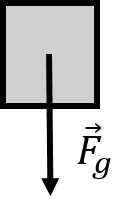
\includegraphics[width=0.1\linewidth]{files/weight-4fe1d7363b0c9d71f9252a9abe66caed.png}
\caption[]{The weight force on an object near the surface of the Earth points towards the centre of the Earth (downwards).}
\label{fig:newtonslaws:weight}
\end{figure}

Although we have not yet introduced the concept of mass, it is worth emphasizing that mass and weight are different (they have different dimensions). Mass is an intrinsic property of an object, whereas weight is a force of gravity that is exerted on that object because it has mass and is located next to another object with mass (e.g. the Earth). On Earth, when we measure our weight, we usually do so by standing on a spring scale, which is designed to measure a force by compressing a spring. We are thus measuring $mg$, which can easily be related to our mass since, on Earth, weight and mass are related by a factor of $g=9.8 {\rm N/kg}$; this is usually what leads to the confusion between mass and weight.

\begin{framed}
\textbf{Checkpoint}\\
A person standing on a scale finds that they weigh $80 {\rm kg}$.

\begin{enumerate}
\item They exert an upwards force on the Earth with a magnitude of $80 {\rm N}$.
\item They exert an upwards force on the Earth with a magnitude of $784 {\rm N}$.
\item They exert an downwards force on the Earth with a magnitude of $80 {\rm N}$.
\item They exert an downwards force on the Earth with a magnitude of $784 {\rm N}$.
\item They exert no force on the Earth.
\end{enumerate}

\begin{framed}
\textbf{Answer}\\
\begin{enumerate}[resume]
\item
\end{enumerate}
\end{framed}
\end{framed}

\subparagraph{Normal forces}

Normal forces are exerted when two surfaces are in contact and ``pushing'' against each other. For example, if a block is resting on a horizontal table, the table will exert a normal force on the block that is upwards. The force is called ``normal'' because it is normal (i.e. perpendicular) to the interface between the two objects. The normal force exerted by a surface onto an object points in the direction \textbf{from the surface to the object} in such a way that it is perpendicular to the interface between the surface and the object. Because of Newton's Third Law, whenever an object experiences a normal force from a surface, the object also exerts a force of the same magnitude (in the opposite direction) on the surface. The magnitude of the normal force exerted by a surface onto an object, in general, depends on the other forces that are exerted on the object. For example, if a block is on a table, it will experience a stronger normal force if you exert a downwards force on the block.

Figure~\ref{fig:newtonslaws:normal} shows two examples of the normal force on a block that is exerted by a surface (it is explicitly assumed that the block also experiences a downwards force from gravity that is not shown). In both cases, the normal force, $\vec N$, is perpendicular to the interface and in the direction that goes from the interface towards the object.

\begin{figure}[!htbp]
\centering
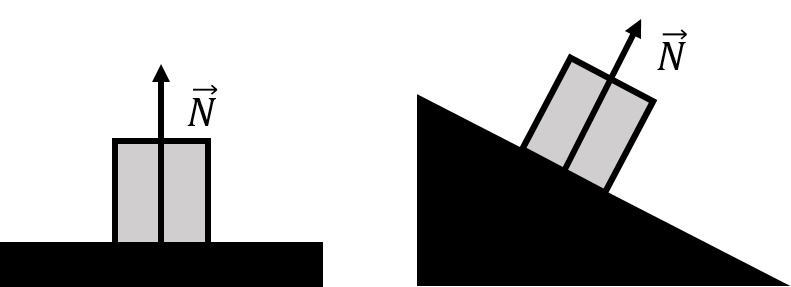
\includegraphics[width=0.5\linewidth]{files/normal-c7095ad7e022213578762c7aadd99feb.png}
\caption[]{The normal force, $\vec N$, exerted by a horizontal surface on a block (left side) and by an inclined surface (right side). In both cases, the normal force on the object is perpendicular to the interface between the object and the surface and points in the direction from the interface towards the object.}
\label{fig:newtonslaws:normal}
\end{figure}

\subparagraph{Frictional forces}

A frictional force can exist at the interface between two surfaces and is always perpendicular to the normal force that corresponds to that interface. A frictional force is used to model the resistance that is felt when one tries to slide an object along a surface. The frictional force is used to model the details of how two surfaces interact at a microscopic level; since surfaces are never perfectly flat, two surfaces will never slide without resistance as the various bumps and valleys of the two surfaces will interact (Figure~\ref{fig:newtonslaws:fsurfaces}). Furthermore, even if the two surfaces were perfectly smooth, the electrons on the two surfaces would still interact and lead to an effective force when one surface moves with respect to the other.

\begin{figure}[!htbp]
\centering
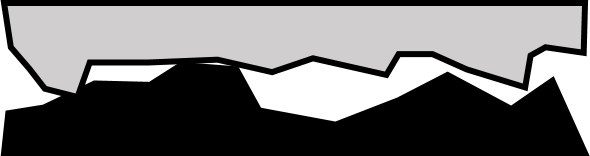
\includegraphics[width=0.3\linewidth]{files/fsurfaces-59ce016a44b5851dc6c2883d2412cfa1.png}
\caption[]{Illustration that the frictional force between surfaces can be thought of as arising from microscopic imperfection in the surfaces, although even two perfectly smooth surfaces would still interact.}
\label{fig:newtonslaws:fsurfaces}
\end{figure}

One distinguishes between two types of frictional forces: kinetic and static, depending on whether the surfaces are sliding with respect to each other (kinetic) or not (static). Because of Newton's Third Law, the objects associated with each surface will both experience a frictional force (same magnitude, opposite direction).

The frictional force exerted on an object is always parallel to the surface of the object. For the kinetic force of friction, the force is exerted in the direction that is opposite to the motion of the object relative to the surface. For the static force of friction, the force is exerted in the direction that is opposite to the \textit{impeding motion}. If a block is sliding towards the right on a table (Figure~\ref{fig:newtonslaws:friction}, left), it will experience a kinetic force of friction that is to the left. The table will then experience a force of friction that is to the right (Newton's Third Law). If there is a heavy crate on the ground which you try to push but does not move (Figure~\ref{fig:newtonslaws:friction}, right), there is a force of static friction exerted by the ground on the object that is in the opposite direction that you are pushing.

\begin{figure}[!htbp]
\centering
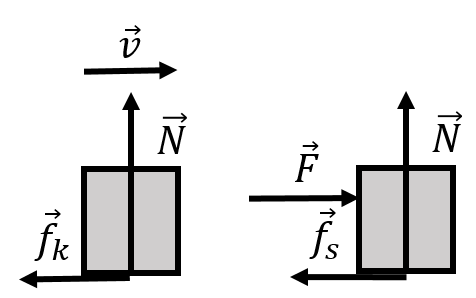
\includegraphics[width=0.5\linewidth]{files/friction-f83362359d4ac6cb10c1abc491c3f88c.png}
\caption[]{(Left:) A block sliding to the right on a horizontal surface (not shown). The force of kinetic friction, $\vec f_k$, is always perpendicular to the normal force and opposite of the direction of motion. (Right:) A block that is being acted upon by an external force $\vec F$ to the right. A force of static friction, $\vec f_s$, is perpendicular to the normal force and opposite the direction of ``impeding motion'' - without the force of static friction, the block would start to accelerate towards the right, so the force of static friction is to the left.}
\label{fig:newtonslaws:friction}
\end{figure}

One key difference between the forces of static and kinetic friction is that the magnitude of the force of static friction can vary in magnitude; the force of static friction on the crate increases as you push harder, until you push hard enough to overcome the maximal force of static friction that can exist between the ground and the crate. Often, the force of kinetic friction is smaller than the static force of friction; you may have noticed that you have to push very hard to get an object sliding, but once it is sliding, you do not need to push as hard to keep it moving.

The magnitude of the kinetic force of friction between two surfaces, $f_k$, is modelled as being proportional to the normal force between the two surfaces:
\begin{equation}
f_k=\mu_kN
\end{equation}
where $\mu_k$ is called the ``coefficient of kinetic friction'' and depends on the two surfaces. If you push down on an object, it is more difficult to slide it along a surface, because the normal force, and thus the kinetic friction force increases.

Similarly, the maximum magnitude of the force of static friction between two surfaces, $f_s$, is modelled as:
\begin{equation}
f_s\leq\mu_sN
\end{equation}
where $\mu_s$ is called the ``coefficient of static friction'' and the inequality sign is used to indicate that the force of static friction has a maximum value, but that its magnitude depends on the other forces being exerted on the object. For example, if you do not push against a crate on a horizontal surface, there is no force of static friction on the crate (as long as no other forces are exerted that are parallel to the surface).

\subparagraph{Tension forces}

Tension forces are ``pulling'' forces that are applied by a rope or other non rigid media (e.g. a chain) which cannot usually be used to push\footnote{If you attached a rigid rod to an object and pulled on the rigid rod, you could call the force exerted by the rod on the object a force of tension, even if the rod is rigid.}. If you attach a rope to a crate and use the rope to pull the crate, we call the force exerted by the rope onto the crate a force of tension.

When you pull on a rope that is attached to a wall at the other end, we say that the rope is under tension, or that the tension force is present throughout the rope. If you pull really hard on the rope, it is harder to displace the centre of the rope (or any other point) than if you did not pull on the rope at all. It thus makes sense to view the tension as being present throughout the rope. The force of tension that a rope can apply onto an object depends on what is pulling on the rope at the other end. A rope can be used to change the direction of a force, as illustrated in Figure~\ref{fig:newtonslaws:tension}, which shows a pulley and rope being used to lift a block vertically by applying a horizontal force, $\vec F$, to the rope.

\begin{figure}[!htbp]
\centering
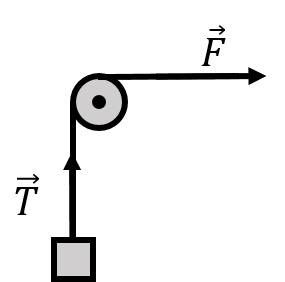
\includegraphics[width=0.25\linewidth]{files/tension-50cd74b547f7e6f7a2b794042bd9b27a.png}
\caption[]{A force $\vec F$ is applied to a rope, which goes around a pulley and is attached to a crate. The rope exerts a force of tension $\vec T$ on the crate. If the pulley and rope are massless, then the magnitude of the applied force is equal to that of the tension force, and the rope and pulley effectively allow one to change the direction of the applied force vector.}
\label{fig:newtonslaws:tension}
\end{figure}

The same tension is present throughout sections of the rope that can move freely. Imagine a rope lying on the ground and someone pressing down with their foot on the rope at its midpoint. If you pull on one end of the rope with your hand, there will be a tension in the section of the rope between your hand and the foot that is pressing on the rope, but the other side of the rope will be slack; the tension is thus different in different sections of the rope. As we will see in later chapters, if a rope goes around a pulley that is accelerating and has mass, then the tension in the rope on either side of the pulley is different; this is similar to the tension being different on either side of the foot pressing down on the rope.

\subparagraph{Drag forces}

Drag forces are exerted on an object that is moving through a fluid (a gas or a liquid). As an object moves through a fluid, the fluid must be displaced which results in a net force opposing the motion of the object. Drag forces are thus always in the opposite direction of the motion of the object relative to the fluid, similar to friction. Often, one hears the term ``air friction'' which refers to the drag force experienced by an object that is moving through the air.

There is no good general model for calculating the magnitude of the drag force on any object moving through any fluid. This usually has to be measured; while good software exist for simulating drag, you will still ultimately need to test your new airplane design in a wind tunnel to measure the drag force.

The magnitude of the drag force generally depends on the cross-section of the object (the area of the object as seen when looking at the object in the direction of motion), the speed of the object, and the visocity of the fluid (how difficult it is to displace the fluid). For small objects moving relatively slowly through a fluid (e.g. pollen falling through the air), the drag force is usually proportional to the object's speed, whereas for larger objects moving faster through a fluid (e.g a car or airplane moving through the air) the drag force is usually proportional to the speed of the object squared.

\subparagraph{Spring forces}

Spring forces are those forces that are exerted by those materials and objects that can be compressed or extended. A common example is a simple coil spring, which has a natural rest length. If the spring is extended, the spring will exert ``restoring forces'' on both ends of the spring that are directed towards the centre of the spring. If the spring is compressed, the spring will exert restoring forces that point away from the centre of the spring. In either case, the spring will exert forces that would allow it to come back to its rest length.

Most springs, if they are not stretched or compressed too much, will exert a restoring force that is given by Hooke's Law:
\begin{equation}
\vec F = -kx \hat x
\end{equation}
where $\vec F$ is the force exerted by the spring, $k$ is called the ``spring constant'' of the spring, and $x$ is the amount that the spring has been stretched or compressed. The negative sign indicates that the restoring force from the spring will be in the opposite direction that the spring length was changed, and the $x$ axis is defined to be co-linear with the axis of the spring and the origin is located where the spring is at rest. This is illustrated in Figure~\ref{fig:newtonslaws:spring}.

\begin{figure}[!htbp]
\centering
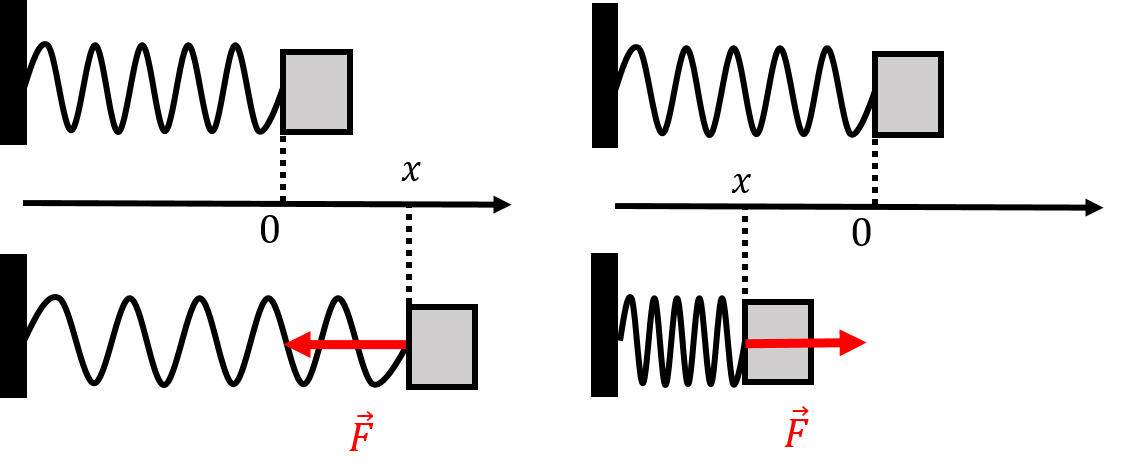
\includegraphics[width=0.7\linewidth]{files/spring-b00122b55ed30b778274a7ba08b20d91.png}
\caption[]{A spring is attached to a fixed wall on its left and to a movable block on its right. The $x$ axis is chosen to describe the position of the end of the spring where the block is attached and the origin corresponds to the point where the spring is not extended or compressed (the top row). The $x$ axis is chosen so that positive values of $x$ correspond to the spring being extended. On the bottom left, the spring is extended by a distance $x$ (the position of the block has positive $x$), and the force from the spring on the block is in the negative $x$ direction. On the bottom right, the spring is compressed (the position of the block has negative $x$), and the force from the spring is in the positive $x$ direction.}
\label{fig:newtonslaws:spring}
\end{figure}

\begin{framed}
\textbf{Checkpoint}\\
In Figure~\ref{fig:newtonslaws:spring}, we chose the positive $x$ axis to correspond to positions where the spring is extended and verified that Hooke's Law ($\vec F= -kx\hat x$) holds. If we had chosen the positive direction to correspond to compression (positive $x$ to the left), would Hooke's Law still correctly describe the direction of the force exerted by the spring on the block?

\begin{enumerate}
\item Yes.
\item No.
\end{enumerate}

\begin{framed}
\textbf{Answer}\\
\begin{enumerate}
\item
\end{enumerate}
\end{framed}
\end{framed}

\subparagraph{Inertial forces}

Inertial forces are exerted on an object when the forces on the object are modelled in a non-inertial frame of reference. For example, in the frame of reference of an accelerating elevator, or that of a car going around a curve, one can use Newton's Three Laws to model motion, if an additional inertial force is included. In a frame of reference that has an acceleration given by $\vec a$, an inertial force $-m\vec a$ is exerted on an object. This is the nature of the outwards force that is felt when your car goes around a curve, or the perception of being weightless in an elevator that has a large downwards acceleration. We will discuss inertial forces in more detail in Section~\ref{sec:newtonslaws:inertialforces}.

\subparagraph{``Applied'' forces}

``Applied'' forces is just a general ``catch-all'' term for specifying forces that are not described above. For example, the force applied by a person onto an object is often referred to as an applied force.

\subsubsection{Mass and inertia}

Mass is a property of an object that quantifies how much matter the object contains. In SI units, mass is measured in kilograms. One kilogram used to be defined to be the mass of a cylinder that is made of a platinum-iridium alloy that is kept at the international Bureau of Weights and Measures, in France. All other masses were obtained by comparison to this standard. In 2019, all base S.I. quantities (such as the kilogram) were redefined based on constants of nature (for example, the kilogram is now defined such that Planck's constant has the exact value $h=6.62607015e -34 {\rm kg\cdot m^2\cdot s^{ -1}}$).

Newton's Second Law introduces the concept of mass as that property of the object that determines how large of an acceleration it will experience given a net force exerted on that object. In principle, one can compare the accelerations of different bodies to that of the international standard to determine their mass in kilograms. For example, under a given net force, if an object's acceleration is half of that of the standard kilogram, the object has a mass of $2 {\rm kg}$.

In the context of Newton's Second Law, mass is a measure of the inertia of an object; that is, it is a measure of how that particular object resists a change in motion due to a force (we can think of a large acceleration as a large change in motion, as the velocity vector of the object will change more). For this reason, the mass that appears in Newton's Second Law is referred to as ``inertial mass''.

As you recall, the weight of an object is given by the mass of the object multiplied by the strength of the gravitational field, $\vec g$. There is no reason that the mass that is used to calculate weight, $F_g=mg$, has to be the same quantity as the mass that is used to calculate inertia $F=ma$. Thus, people will sometimes make the distinction between ``gravitational mass'' (the mass that you use to calculate weight and the force of gravity) and ``inertial mass'' as described above. Very precise experiments have been carried out to determine if the gravitational and inertial masses are equal. So far, experiments have been unable to detect any difference between the two quantities. As we will see, both Newton's Universal Theory of Gravity and Einstein Theory of General Relativity assume that the two are indeed equal. In fact, it is a key requirement for Einstein's Theory that the two be equal (the assumption that they are equal is called the ``Equivalence Principle''). You should however keep in mind that there is no physical reason that the two are the same, and that as far as we know, it is a coincidence!

Unless stated otherwise, we will not make any distinction between gravitational and inertial mass and assume that they are equal. We will simply use the term ``mass'' and only clarify the type of mass when relevant (e.g. when we cover gravity).

\subsubsection{Exploring Forces with PhET}

In the PhET simulation below, choose the ``Motion'' tab to start the simulation. Make sure the boxes that say ``Force'', ``Values'' and ``Speed'' are checked!

\paragraph{Newton's First Law}

Apply a force of 50 N right to the box. Describe the motion while the force is exerted of the box using physics terms (i.e. velocity, acceleration, displacement). Refer to the speedometer in your answer.
Reset the scenario (don't forget to check forces, speed again). Apply a force of 50 N to the right for about 5 seconds then reduce the applied force to zero (the ``dummy'' should stop pushing). Don't reset the scenario. Describe the motion of the box. Refer to the speedometer in your answer.
Apply a force of 50N to the left. Describe the motion of the box.
With the box moving at constant velocity. Explain the exact steps needed to make the box come to a stop. Do this for two different stopping forces and explain the differences.

\subparagraph{Summary}

Newton's First Law of Motion States ``An object at rest stays at rest and an object in motion stays in motion with the same speed and in the same direction unless acted upon by an unbalanced force.'' Explain how your observations above support this Law.

\begin{figure}[!htbp]
\centering
\caption[]{PhET simulation to model forces and motion.}
\label{phet:newtonslaws:ForcesAndMotion}
\end{figure}

\paragraph{Newton's Second Law}

Reset the sim, don't forget to check force, values and speed again. Remove the box and place a garbage can on top of the skateboard. Using a timer (on your phone, for example), measure the amount of time it takes to reach maximum speed using a force of 50 N. Try this again with forces of 100N, and 200N. Enter your results in a table like the one below.

\begin{table}
\centering
\caption[]{A table to record observations from PhET simulation.}
\label{table:newtonslaws:phetsim}
\begin{tabular}{p{\dimexpr 0.333\linewidth-2\tabcolsep}p{\dimexpr 0.333\linewidth-2\tabcolsep}p{\dimexpr 0.333\linewidth-2\tabcolsep}}
\toprule
Applied Force (N) & Time to Max Speed (s) & Acceleration (m/s2) \\
\hline
50 &  &  \\
100 &  &  \\
200 &  &  \\
\bottomrule
\end{tabular}
\end{table}

The maximum velocity is 40 m/s. Can you determine the acceleration of each applied force using the definition of acceleration  $a=\Delta v/\Delta t$? Can you determine the mass of the trash can and skateboard using Newton's 2nd Law,  $F=ma$?

\subparagraph{Trends}

In Excel, plot force on the y-axis and acceleration on the x-axis. Add a linear trendline, and show the equation. How does the value of the slope compare to the mass you calculated? Can you explain this?

\subparagraph{Summary}

Newton's Second Law states ``The acceleration of an object as produced by a net force is directly proportional to the magnitude of the net force, in the same direction as the net force, and inversely proportional to the mass of the object.'' Explain how your observations above support this Law.

\paragraph{Frictional Effects}

The behavior of the skateboard in Part I and part II were not very realistic because friction was not present. At the bottom of the screen is a simulation that includes friction. Select this simulation.

\begin{enumerate}
\item Set friction to ``none''. Notice how the screen changed. Why do you think the app designers did that?
\item Make sure that only speed box is checked.\begin{itemize}
\item Apply a force to get the box to about half of it's maximum speed, then remove the force.
\item While the box is moving, move the friction slider to 1/2 way.
\end{itemize}
\end{enumerate}

What happened to the box?

\subparagraph{Summary}

Is friction a force? What evidence do you have?

\paragraph{Friction and Newton's Second Law}

Reset the Friction app. Make sure Forces and Speed are checked.

\begin{enumerate}
\item Apply a force of 50 N. Describe the movement of the box.
\item Apply a force of 100 N. Describe the movement of the box.
\item Apply a force of 150 N. Describe the movement of the box.
\item Check the box that says ``Sum of Forces''. Repeat procedures 1, 2, and 3. What was different about 3?
\end{enumerate}

\subparagraph{Summary}

Newton's Second Law states ``The \textbf{acceleration of an object as produced by a net force} is directly proportional to the magnitude of the net force, \textbf{in the same direction as the net force}, and inversely proportional to the mass of the object.'' Explain how your observations relate to the underlined portion of this Law (hint, you might want to look up the definition of the word ``net'').

\subsubsection{Applying Newton's Laws}

Now that we have introduced all of the concepts from Newton's Theory of Classical Physics, we present some general strategies for building models that use the theory. Recall that if we can describe the motion of all objects of interest to us, we have described everything that we can. Newton's Second Law allows us to determine the acceleration of an object based on the net force acting on the object. Once we have determined the accelerations of all objects of interest we have built a complete model.

The most important step in applying Newton's Theory is to identify the forces that are exerted on an object. The most important step in applying Newton's Theory is to identify the forces that are exerted on an object. The most important step in applying Newton's Theory is to identify the forces that are exerted on an object. Now that you have read it three times, you realize this step is important, right?!

The strategy for building a model for the motion of an object using Newton's Theory is straightforward:

\begin{enumerate}
\item Identify an inertial frame of reference in which to build the model.
\item Identify the forces acting on the object (did we mention that this step is important?).
\item Draw a free-body diagram.
\item Apply Newton's Second Law.
\end{enumerate}

\paragraph{Identifying the forces}

The first step in applying Newton's theory is to identify all of the forces that are acting on an object. This can be done by asking yourself: ``what could possibly be pushing or pulling on the object?'', as well as running through the list of forces that we enumerated in Section~\ref{sec:newtonslaws:typesofforces} to identify if any of them are relevant here. For easy reference, we reproduce the types of forces here and include some questions that you might ask yourself to decide whether or not to include the corresponding force:

\begin{itemize}
\item Weight (is the object near the surface of a planet?).
\item Normal forces (is the object in contact with any surface? There could be more than one!).
\item Frictional forces (are there static or kinetic friction forces associated with the normal forces?).
\item Tension forces (is something like a rope pulling on the object?).
\item Drag forces (is the object moving through a fluid?).
\item Spring forces (is there a spring pushing or pulling on the object?).
\item Applied forces (is anything else pushing or pulling on the object?).
\end{itemize}

\begin{framed}
\textbf{Example 5.1}\\
\begin{figure}[!htbp]
\centering
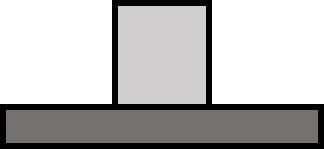
\includegraphics[width=0.2\linewidth]{files/blockH-37f13335eeee7e4dfbf9e4e15d1d06e2.png}
\caption[]{A block on a horizontal table.}
\label{fig:newtonslaws:blockH}
\end{figure}

A block of mass $m$ is at rest on a horizontal table, as shown in Figure~\ref{fig:newtonslaws:blockH}. What forces are exerted on the block?

\begin{framed}
\textbf{Solution}\\
The forces on the block are illustrated in Figure~\ref{fig:newtonslaws:blockH_forces} and are:

\begin{enumerate}
\item $\vec F_g$, its weight.
\item $\vec N$, a normal force exerted by the plane. The normal force is perpendicular to the interface between the table and the block. It points upwards in ``reaction'' to the downwards force that the block exerts onto the table. The downwards force from the block onto the table is not shown, since that force is not exerted on the block but on the table.
\end{enumerate}

\begin{figure}[!htbp]
\centering
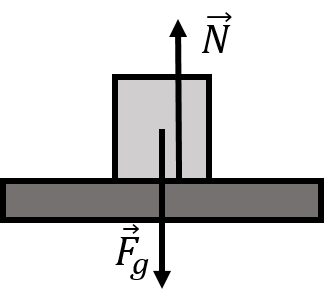
\includegraphics[width=0.2\linewidth]{files/blockH_forces-9de9eaa73395c6a6eec19d08d59ee2a0.png}
\caption[]{Forces on a block on a horizontal table.}
\label{fig:newtonslaws:blockH_forces}
\end{figure}
\end{framed}
\end{framed}

\begin{framed}
\textbf{Example 5.2}\\
\begin{figure}[!htbp]
\centering
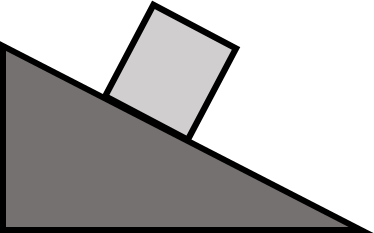
\includegraphics[width=0.2\linewidth]{files/blockI-3db8645a1af042fb7c6876e81faf123a.png}
\caption[]{A block on an inclined surface.}
\label{fig:newtonslaws:blockI}
\end{figure}

A block of mass $m$ is at rest on a inclined surface, as shown in Figure~\ref{fig:newtonslaws:blockI}. What forces are exerted on the block?

\begin{framed}
\textbf{Solution}\\
The forces on the block are illustrated in Figure~\ref{fig:newtonslaws:blockI_forces} and are:

\begin{enumerate}
\item $\vec F_g$, its weight.
\item $\vec N$, a normal force exerted by the inclined plane.
\item $\vec f_s$, a force of static friction exerted by the inclined plane. Without this force, the block would slide down. The force is in the direction opposite of impeding motion and is parallel to the interface (and perpendicular to the normal force).
\end{enumerate}

\begin{figure}[!htbp]
\centering
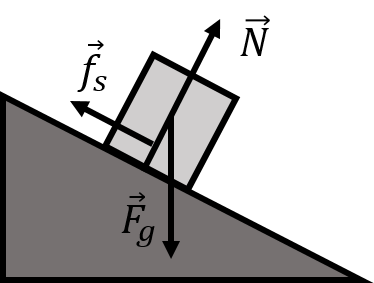
\includegraphics[width=0.2\linewidth]{files/blockI_forces-afd3e702cb9372b2d1e26821e36eaefc.png}
\caption[]{Forces on block on an inclined surface.}
\label{fig:newtonslaws:blockI_forces}
\end{figure}
\end{framed}
\end{framed}

\begin{framed}
\textbf{Example 5.3}\\
\begin{figure}[!htbp]
\centering
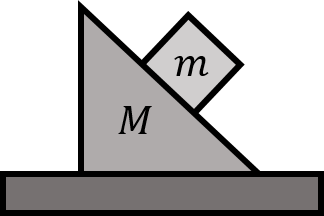
\includegraphics[width=0.2\linewidth]{files/2blockswedge-cc05d5d048b82edd0d9d05a6f393ea62.png}
\caption[]{A block resting on a wedge-shaped block.}
\label{fig:newtonslaws:2blockswedge}
\end{figure}

A block of mass $m$ is at rest on a wedge-shaped block of mass $M$ itself at rest on a horizontal table, as shown in Figure~\ref{fig:newtonslaws:2blockswedge}. What forces are exerted on each of the two blocks?

\begin{framed}
\textbf{Solution}\\
Since it will be too messy to draw all of the forces on the same diagram, we have drawn each block separately in Figure~\ref{fig:newtonslaws:2blockswedge_forces}.
Usually, when multiple blocks are stacked on each other, it is easiest to start with the forces on the top block. In this case, the top block is in the same condition as the block from Example~5.2. The forces exerted on the top block are:

\begin{enumerate}
\item $\vec F_g^m$, its weight.
\item $\vec N^m$, a normal force from the wedge-shaped block.
\item $\vec f_s^m$, a force of static friction exerted by the wedge-shaped block.
\end{enumerate}

The forces exerted on the wedge-shaped block are:

\begin{enumerate}
\item $\vec F_g^M$, its weight.
\item $\vec N^M$, a normal force exerted by the small block. Note that this force is equal in magnitude and opposite in direction to $\vec N^m$ (the two forces, $\vec N^m$ and $\vec N^M$, which are on different objects, are an action/reaction pair of forces).
\item $\vec f_s^M$, a force of friction exerted by the small block (again, this forms an action/reaction pair of forces with  $\vec f_s^m$).
\item $N_2^M$, a normal force exerted by the table.
\end{enumerate}

The forces for both blocks are shown in Figure~\ref{fig:newtonslaws:2blockswedge_forces}.

\begin{figure}[!htbp]
\centering
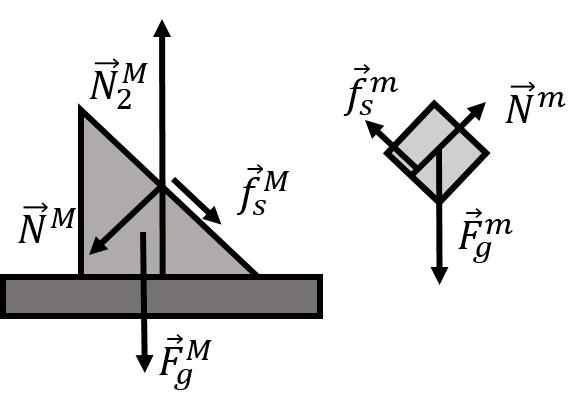
\includegraphics[width=0.4\linewidth]{files/2blockswedge_forces-5138bb9428de3882b524b92d121f8b64.png}
\caption[]{Forces on the block and the wedge-shaped block.}
\label{fig:newtonslaws:2blockswedge_forces}
\end{figure}
\end{framed}
\end{framed}

\paragraph{Free body diagrams}

In order to analyse the forces on an object more clearly, it is a very good idea to draw a ``Free-Body Diagram'' (FBD). A free-body diagram is simply a diagram where we draw the forces on a single object and represent the object as a point. Because the object is a point, we do not worry where on the object the forces are exerted. In later chapters, we will see that for extended bodies, it does matter where the forces are applied. However, Newton's Laws as presented so far are only valid for objects that can be represented as a small point.

\begin{figure}[!htbp]
\centering
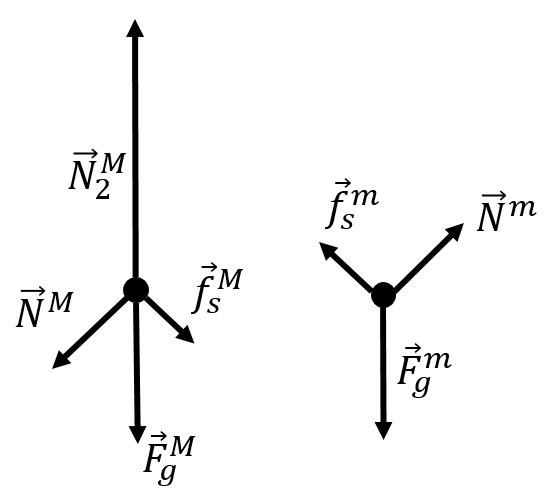
\includegraphics[width=0.5\linewidth]{files/2blockswedge_fbd-3e88aaa142b1532dd88ad2089c06532d.png}
\caption[]{Free-body diagram for the block and the wedge-shaped block from Figure~\ref{fig:newtonslaws:2blockswedge}.}
\label{fig:newtonslaws:2blockswedge_fbd}
\end{figure}

In Figure~\ref{fig:newtonslaws:2blockswedge} above, we would draw one free-body diagram for each object (each mass), as shown in Figure~\ref{fig:newtonslaws:2blockswedge_fbd}.

\begin{framed}
\textbf{Example 5.4}\\
\begin{figure}[!htbp]
\centering
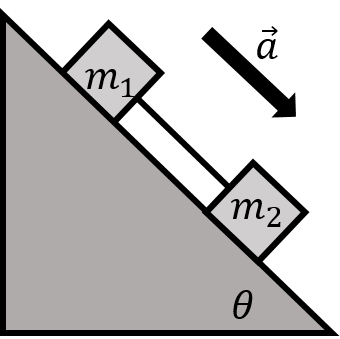
\includegraphics[width=0.2\linewidth]{files/2blocksI-3c13a2d5a477e53026e27df46a6b9d2a.png}
\caption[]{Two connected blocks sliding down an inclined plane.}
\label{fig:newtonslaws:2blocksI}
\end{figure}

Two blocks, of masses $m_1$ and $m_2$, are placed on an inclined plane that makes an angle $\theta$ with the horizontal. The blocks are connected by a massless string, as shown in Figure~\ref{fig:newtonslaws:2blocksI}. The two blocks are sliding and accelerating downwards with an acceleration, $\vec a,$ as shown. The coefficient of kinetic friction between the plane and either block is $\mu_k$. Draw a free-body diagram for each block.

\begin{framed}
\textbf{Solution}\\
First, we identify the forces on each mass (each block), which we then use to make the free-body diagram shown in Figure~\ref{fig:newtonslaws:2blocksI_fbd}. On mass $m_1$, the forces are:

\begin{enumerate}
\item $\vec F_{g1}$, its weight.
\item $\vec N_1$, a normal force exerted by the inclined plane.
\item $\vec f_{k1}$, a force of kinetic friction exerted by the inclined plane. The force is in the opposite direction of the motion, and has a magnitude given by $f_{k1}=\mu_kN_1$.
\item $\vec T$, a force of tension from the string.
\end{enumerate}

On mass $m_2$, the forces are:

\begin{enumerate}
\item $\vec F_{g2}$, its weight.
\item $\vec N_2$, a normal force from the inclined plane.
\item $\vec f_{k2}$, a force of kinetic friction exerted by the inclined plane. The force is in the opposite direction of the motion, and has a magnitude given by $f_{k2}=\mu_kN_2$.
\item $-\vec T$, a force of tension from the string. This is the same force as on $m_1$, but in the opposite direction. We chose to label the force as $-\vec T$, instead of using a different variable, since it is just the negative of the vector that represents the tension force on $m_1$.
\end{enumerate}

In Figure~\ref{fig:newtonslaws:2blocksI_fbd}, we have shown the forces on each block using a free-body diagram. We also reproduced the vector for the acceleration (we drew the vector for the acceleration using a thicker arrow to indicate that it has a different dimension). We also reproduced the angle $\theta$ in the free-body diagram, as this is helpful once the free-body diagram is used with Newton's Second Law.

\begin{figure}[!htbp]
\centering
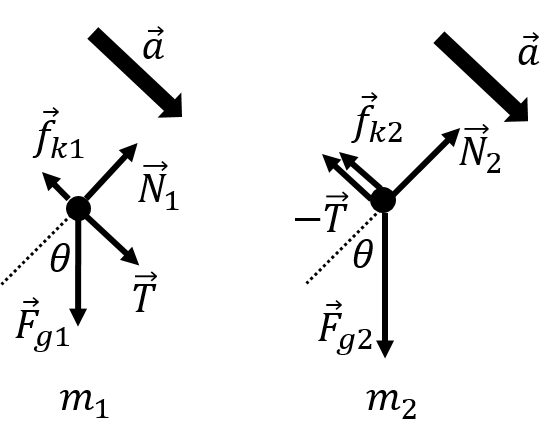
\includegraphics[width=0.5\linewidth]{files/2blocksI_fbd-f77c2b42d2da1e66c936f771cec3aa4d.png}
\caption[]{Free-body diagram for the blocks $m_1$ and $m_2$ from Figure~\ref{fig:newtonslaws:2blocksI}}
\label{fig:newtonslaws:2blocksI_fbd}
\end{figure}
\end{framed}
\end{framed}

\paragraph{Using Newton's Second Law}

Applying Newton's Second Law is straightforward once all of the forces exerted on an object have been identified. You should thus make sure that you spend most of your time drawing a good and complete free-body diagram before proceeding.

Newton's Second Law is a vector equation that relates the vector sum of all forces exerted on an object and the acceleration vector of the object. This corresponds to one scalar equation per component of the vector.

\begin{equation}
\sum \vec F &=m\vec a\\
\sum F_x &= ma_x \\
\sum F_y &= ma_y \\
\sum F_z &= ma_z
\end{equation}
In order to use Newton's Second Law, we thus need to introduce a coordinate system so that we can work with the components of the vectors (forces and acceleration) in that coordinate system. Usually, a good choice of coordinate system is one where the $x$ (or $y$) axis is parallel to the acceleration vector. Figure~\ref{fig:newtonslaws:2blocksI_fbd_m1} shows the free-body diagram from the $m_1$ block from the previous example (Example~5.4) along with a good choice of coordinate system.

\begin{figure}[!htbp]
\centering
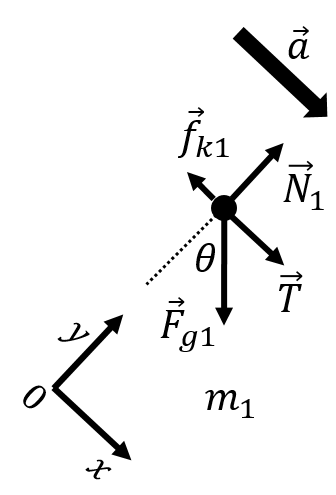
\includegraphics[width=0.25\linewidth]{files/2blocksI_fbd_m1-dfad6a15fa92ed9e9ade622ff20be11f.png}
\caption[]{Free-body diagram and choice of coordinate system for the $m_1$ blocks from Figure~\ref{fig:newtonslaws:2blocksI_fbd}}
\label{fig:newtonslaws:2blocksI_fbd_m1}
\end{figure}

To apply Newton's Second Law using the free-body diagram and coordinate system from Figure~\ref{fig:newtonslaws:2blocksI_fbd_m1}, we first write out all of the vector and then identify their $x$ and $y$ components. The force vectors are:
\begin{equation}
\vec T &= T\hat x+0\hat y\\
\vec f_{k1}&=-f_{k1}\hat x+0\hat y\\
\vec F_{g1}&=m_1g(\sin\theta \hat x-\cos\theta \hat y)\\
\vec N_1&=0\hat x+N_1\hat y
\end{equation}
We can now write out the $x$ component of Newton's Second Law:
\begin{equation}
\sum F_x = T-f_{k1}+F_{g1}\sin\theta &= m_1 a\\
\therefore T-f_{k1}+F_{g1}\sin\theta &= m_1 a
\end{equation}
where we note that the normal force has no component in the $x$ direction. The $y$ component of Newton's Second Law for mass $m_1$ is given by:
\begin{equation}
\sum F_y = N_1-F_{g1}\cos\theta&=0\\
\therefore N_1-F_{g1}\cos\theta&=0
\end{equation}
where we note that the forces of tension and friction have no $y$ component. The two equations that we obtained above for $x$ and $y$ fully specify the motion of the $m_1$ block if all quantities are known\footnote{Since we have two equations, we technically only need to specify all but two quantities to be able to fully model the motion of the block.}.

A few notes on applying Newton's Second Law:

\begin{itemize}
\item When applying Newton's Second Law, analyze each mass in the problem separately. It does not matter that block $m_1$ is connected by a rope to block $m_2$. Once you have determined all of the forces exerted on $m_1$, you can write Newton's Second Law for $m_1$.
\item Newton's Second Law is a vector equation; this means that it is true for each (scalar) component of the vectors involved.
\item You can choose the coordinate system, so choose one that makes it easy to write out the vector components. A good choice is to choose $x$ to be parallel to the acceleration vector, so that you do not have to break the acceleration vector up into components. The choice of coordinate system is only made in order to allow you to write out the components of Newton's Second Law based on the free-body diagram.
\item Treat each mass separately (since Newton's Second Law is only true for an individual mass). This means that each mass will have its own free-body diagram and that you can choose the coordinate system that is most convenient for a given free-body diagram. In particular, this means that you do not need to choose the same coordinate system for different masses in a problem.
\end{itemize}

The following example shows how to write Newton's Second Law for a system of two blocks.

\begin{framed}
\textbf{Example 5.5}\\
\begin{figure}[!htbp]
\centering
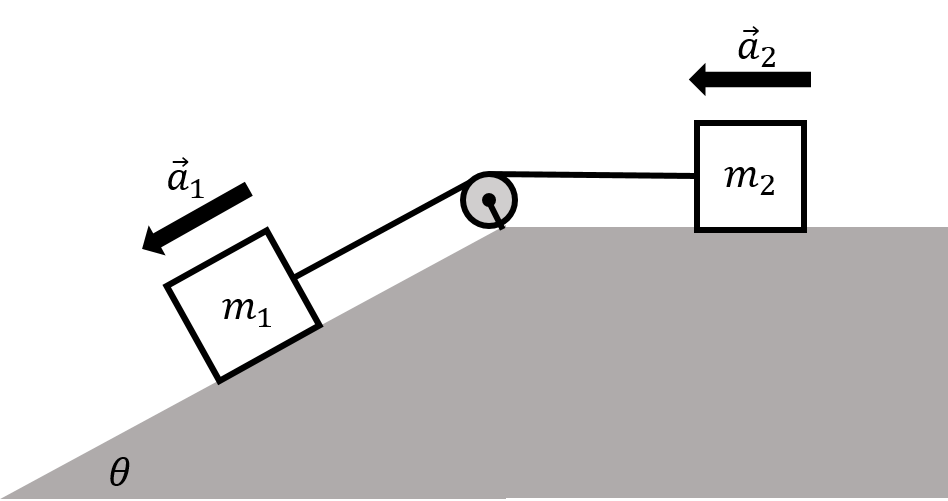
\includegraphics[width=0.6\linewidth]{files/2blocksHI-c8b3543b2031065c3e6b1ad099f2a512.png}
\caption[]{Two blocks connected by a massless string and massless pulley. Both blocks are accelerating.}
\label{fig:newtonslaws:2blocksHI}
\end{figure}

A block of mass $m_1$ is placed on an incline that makes an angle of $\theta$ with the horizontal. The block of mass $m_1$ is connected by a massless string through a massless pulley to a second block of mass $m_2$, which rests on a horizontal surface. The blocks are accelerating in such a way that the block of mass $m_1$ is accelerating down the incline, as shown in Example~5.5. The coefficient of kinetic friction between either block and the surface it is resting on is $\mu_k$. Write Newton's Second Law for both blocks.

\begin{framed}
\textbf{Solution}\\
First, we identify the forces on each mass (each block). On mass $m_1$, the forces are:

\begin{enumerate}
\item $\vec F_{g1}$, its weight.
\item $\vec N_1$, a normal force exerted by the inclined plane.
\item $\vec f_{k1}$, a force of kinetic friction exerted by the inclined plane. The force is in the opposite direction of the motion, and has a magnitude given by $f_{k1}=\mu_kN_1$.
\item $\vec T_1$, a force of tension from the string.
\end{enumerate}

On mass $m_2$, the forces are:

\begin{enumerate}
\item $\vec F_{g2}$, its weight.
\item $\vec N_2$, a normal force from the horizontal surface.
\item $\vec f_{k2}$, a force of kinetic friction exerted by the horizontal surface. The force is in the opposite direction of the motion, and has a magnitude given by $f_{k2}=\mu_kN_2$.
\item $\vec T_2$, a force of tension from the string. This force has the same magnitude as the tension force $\vec T_1$ exerted on mass $m_1$, because the pulley is massless.
\end{enumerate}

We can then proceed to draw the free-body diagram for each mass, and use that to write out Newton's Second Law. For mass $m_1$, the free-body diagram is shown in Figure~\ref{fig:newtonslaws:2blocksHI_fbd_m1}. We have chosen a coordinate system that has the $x$ axis parallel to the acceleration of the block, and the $y$ axis upwards and perpendicular to the $x$ axis, as shown.

\begin{figure}[!htbp]
\centering
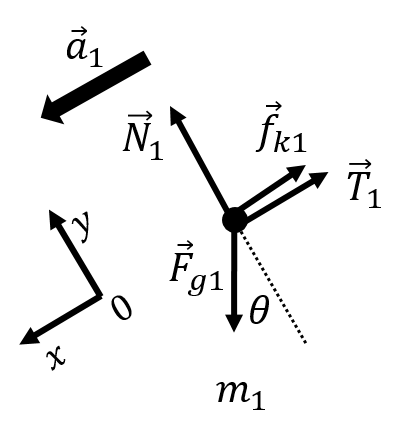
\includegraphics[width=0.25\linewidth]{files/2blocksHI_fbd_m1-592fdf3eded285cafdfcf490baa01fff.png}
\caption[]{Free-body diagram for $m_1$.}
\label{fig:newtonslaws:2blocksHI_fbd_m1}
\end{figure}

For $m_1$, we can write Newton's Second Law, starting with the $x$ components:
\begin{equation}
\sum F_x = F_{g1}\sin\theta-f_{k1}-T_1&=m_1a_1\\
\therefore m_1 g\sin\theta -\mu_k N_1 - T_1 &= m_1 a_1
\end{equation}
where, in the second line, we used the magnitude of the weight ($F_{g1}=m_1g$) and of the force of kinetic friction ($f_{k1}=\mu_kN_1$). For the $y$ component of Newton's Second Law, in which the acceleration has no component, we have:
\begin{equation}
\sum F_y = N_1 - F_{g1}\cos\theta &= 0\\
\therefore N_1=m_1g\cos\theta
\end{equation}
which shows us that the magnitude of the normal force can easily be expressed in terms of the weight ($F_{g1}=m_1g$) and the angle of the incline.

For $m_2$, we can proceed in much the same way, choosing a different coordinate system, since the acceleration vector for $m_2$ points in a different direction (we don't have to choose a different coordinate system, but we can if we find it makes things easier). The free-body diagram for $m_2$ is shown in Figure~\ref{fig:newtonslaws:2blocksHI_fbd_m2} along with our choice of coordinate system.

\begin{figure}[!htbp]
\centering
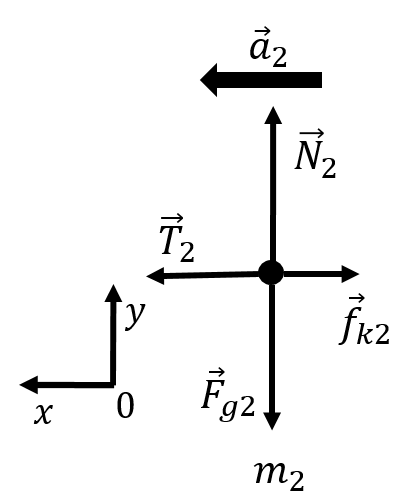
\includegraphics[width=0.25\linewidth]{files/2blocksHI_fbd_m2-e2f7cebc9fb5ec0eecb008050ba5906d.png}
\caption[]{Free-body diagram for $m_2$.}
\label{fig:newtonslaws:2blocksHI_fbd_m2}
\end{figure}

We start by writing out the $x$ component of Newton's Second Law for $m_2$:
\begin{equation}
\sum F_x = T_2 - f_{k2} &= m_2 a_2\\
\therefore T_2 - \mu_k N_2 = m_2 a_2
\end{equation}
where again, we expressed the kinetic force of friction using the normal force and the coefficient of kinetic friction. The $y$ component of Newton's Second Law gives:
\begin{equation}
\sum F_y = N_2 - F_{g2} &=0\\
\therefore N_2 = m_2g
\end{equation}
where again, we expressed the weight in terms of the mass and $g$, and we find that the normal force has the same magnitude as the weight.

Now that we have written Newton's Second Law \textbf{for each mass}, we can write all four equations that we obtained to describe \textbf{the system of two masses}. We should also note that the magnitude of the tension forces are the same for the two masses ($T_1=T_2=T$), and that since the masses are connected by a string, the magnitude of their acceleration vectors are the same ($a_1=a_2=a$). Using this, we can describe the full system with the following 4 equations:
\begin{equation}
m_1 g\sin\theta -\mu_k N_1 - T &= m_1 a\\
N_1=m_1g\cos\theta\\
T - \mu_k N_2 = m_2 a\\
N_2 = m_2g
\end{equation}
Of the variables above ($m_1$, $m_2$, $\mu_k$, $T$, $N_1$, $N_2$, $a$), one would only need to specify all but four of them to fully describe the motion of the system. For example, if one specifies the two masses and the coefficient of kinetic friction, all of the other variables can be determined.
\end{framed}
\end{framed}

\subsubsection{The acceleration due to gravity}

If you have studied some physics before reading this textbook, you may have been surprised by our choice of dimension for $g$ to be force per unit mass rather than acceleration. This is indeed an unconventional choice as $g$ is usually presented as ``the acceleration due to Earth's gravity'' instead of the ``strength of Earth's gravitational field''. Our choice comes from the potential difference between inertial mass, $m_I$, and gravitational mass, $m_G$, which we distinguish in this section.

Consider the simple model of a mass falling freely near the surface of the Earth in the absence of air-resistance. The only force exerted on the mass is its weight, $m_G\vec g$, which is given in terms of gravitational mass (the mass that determines how an object experiences gravity). Both the weight and the acceleration of the object point downwards. The free-body diagram for the mass is shown in Figure~\ref{fig:newtonslaws:gravity_fbd}, where the $y$ axis was chosen to be vertically upwards (co-linear with the acceleration).

\begin{figure}[!htbp]
\centering
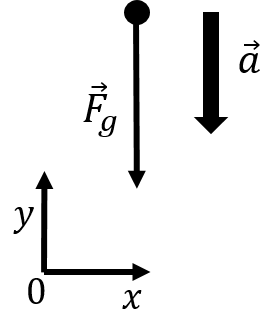
\includegraphics[width=0.2\linewidth]{files/gravity_fbd-c30c31a677237e1182803a455338a61b.png}
\caption[]{Free-body diagram for a mass that is free-falling in the absence of air resistance (drag).}
\label{fig:newtonslaws:gravity_fbd}
\end{figure}

Writing out the $y$ component of Newton's Second Law, being careful to distinguish between inertial and gravitational mass, and noting that both the weight and the acceleration are in the negative $y$ direction:
\begin{equation}
\sum F_y = -F_g &= -m_I a\\
\therefore m_Gg &= m_I a
\end{equation}
This makes it clear that $g$ is not necessarily the acceleration due to gravity. It is only the acceleration due to gravity in the limit that the inertial and gravitational masses are the same. If $m_G=m_I$, then we have:
\begin{equation}
a = g
\end{equation}
and indeed, the acceleration of objects near the surface of the Earth has a magnitude of $g$. It is also clear that the dimensions of $g$ can also be written as an acceleration, and in most cases, one writes that, near the surface of the Earth, $g=9.8 {\rm m/s^2}$. You should however remember that this is only true when inertial and gravitational masses are the same, and that $g$ really should be thought of as the strength of the gravitational field, not as an acceleration.

\subsubsection{Non-inertial frames of reference and inertial forces}\label{sec:newtonslaws:inertialforces}

In the previous sections, we described how to use Newton's First Law to identify an inertial frame of reference (one where Newton's First Law holds true) in order to identify the forces exerted on an object so that Newton's Second Law could be applied. It is possible to apply Newton's Laws in a non-inertial frame of reference, \textbf{provided that one includes an additional ``inertial force''.}

Let us assume that we hang a mass, $m$, from the ceiling of our car using a string. If the car accelerates forwards with a constant acceleration, $\vec a$, the mass will swing towards the back of the car and the string will not be vertical as long as the car maintains its constant acceleration, as shown in Figure~\ref{fig:newtonslaws:car}. As the car maintains its acceleration, the hanging mass will not move relative to the car.

\begin{figure}[!htbp]
\centering
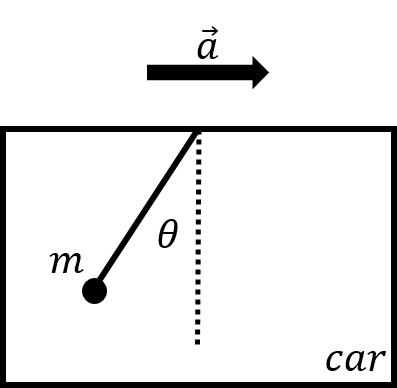
\includegraphics[width=0.3\linewidth]{files/car-d6de3b6fb6dc959ca9eb8cbda22e5819.png}
\caption[]{A mass hanging from the ceiling of a car accelerating to the right.}
\label{fig:newtonslaws:car}
\end{figure}

We can analyse this motion from the inertial frame of reference of the ground. In this frame of reference, there are two forces exerted on the mass:

\begin{enumerate}
\item $\vec F_g$, its weight, with magnitude $mg$.
\item $\vec T$, a force of tension exerted by the string, in the direction of the string.
\end{enumerate}

The two forces are shown in the free-body diagram of Figure~\ref{fig:newtonslaws:car_fbd}, along with a coordinate system chosen such that $x$ points in the direction of the acceleration the mass (which is the same as the acceleration of the car, since the mass does not move relative to the car).

\begin{figure}[!htbp]
\centering
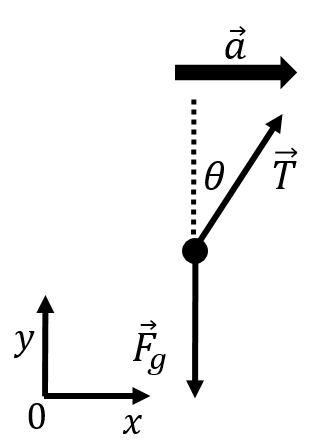
\includegraphics[width=0.2\linewidth]{files/car_fbd-208c42cf97f9c8102e97d3a05c5d8e7c.png}
\caption[]{Free-body diagram for the forces acting on a mass suspended from the ceiling of accelerating car.}
\label{fig:newtonslaws:car_fbd}
\end{figure}

Writing out the $x$ and $y$ components of Newton's Second Law for the mass, we have:
\begin{equation}
\sum \vec F &= \vec T + \vec F_g= m \vec a\\
\therefore\sum F_x &= T\sin\theta = ma\\
\therefore\sum F_y &= T\cos\theta-F_g=0
\end{equation}
We can, instead, model the motion of the mass in the frame of reference of the car, by pretending that we are sitting in the car. In the frame of reference of the car, the mass is immobile, and thus has no acceleration. In the non-inertial frame of reference of the car, we still have the weight and tension forces exerted on the mass; these have the same magnitude and direction as in the inertial frame of reference of the ground. One could replace the string with a spring scale, and observers in the car and on the ground would agree that the spring scale reads the same number. Those observers would also agree that the weight of the mass is the same. However, the two observers disagree on whether the mass is accelerating, since the observer in the car measures that the mass has no acceleration.

In the frame of reference of the car, the acceleration of the mass is zero. If we want Newton's Second Law to hold, this implies that, in the reference frame of the car, the sum of the forces on the mass must be zero:
\begin{equation}
\sum \vec F & = 0\quad\quad\text{(car reference frame)}
\end{equation}
We know from analysing the motion from the frame of reference of the ground that the vector sum of the forces $\vec T$ and $\vec F_g$ is equal to $m\vec a$. The only way for the force in the frame of reference of the car to add up to zero is if there is an additional force, $\vec F_I$, that is exerted in that frame of reference:
\begin{equation}
\sum \vec F &= \vec T + \vec F_g + \vec F_I =0\quad\quad\text{(car reference frame)}
\end{equation}
Since we know that $\vec T + \vec F_g=m\vec a$, we can substitute this in the equation above:
\begin{equation}
\sum \vec F &= \vec T + \vec F_g + \vec F_I =0\quad\quad\text{(car reference frame)}\\
&=m\vec a+\vec F_I = 0\\
\therefore F_I &= -m\vec a
\end{equation}
and we find that this ``inertial force'', $\vec F_I$, must be exerted in the opposite direction from the acceleration of the frame of reference, with a magnitude given by $ma$. The free-body diagram for the mass, as viewed in the reference frame of the car, is illustrated in Figure~\ref{fig:newtonslaws:car_fbd2}.

\begin{figure}[!htbp]
\centering
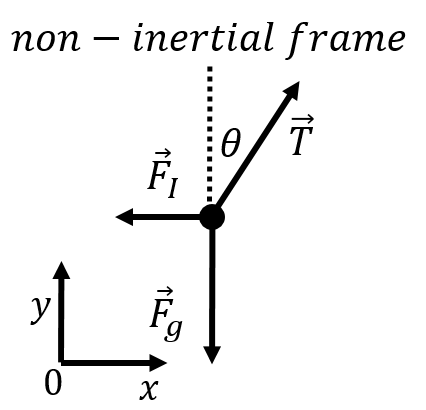
\includegraphics[width=0.3\linewidth]{files/car_fbd2-33f824af64e43fd4a4fff2626544ecca.png}
\caption[]{Free-body diagram for the forces acting on a mass suspended from the ceiling of accelerating car, in the frame of reference of the car. An additional inertial force, $\vec F_I= -m\vec a$, has to be included.}
\label{fig:newtonslaws:car_fbd2}
\end{figure}

\begin{framed}
\textbf{Example 5.6}\\
You are in an elevator that is accelerating downwards with a constant acceleration $\vec a$. You are standing on a spring scale. What is the value of your weight as displayed on the spring scale? Assume that your mass is $m$. (The spring scale will display your weight as having the same magnitude as the normal force that the scale exerts on you).

\begin{framed}
\textbf{Solution}\\
We can model your motion in the non-inertial frame of reference of the elevator, where your acceleration is zero. The forces that are exerted on you are:

\begin{enumerate}
\item $\vec F_g$, your weight, with magnitude $mg$.
\item $\vec N$, the normal force exerted upwards by the spring scale, which is the weight as measured by the scale.
\item $\vec F_I$, an inertial force with magnitude $ma$ that is exerted upwards (in the direction opposite of the acceleration of the frame of reference).
\end{enumerate}

The forces in the frame of reference of the elevator are illustrated in Figure~\ref{fig:newtonslaws:elevator_fbd}, along with a coordinate system that was chosen so that the forces are co-linear with one of the axes (since the acceleration is zero).

\begin{figure}[!htbp]
\centering
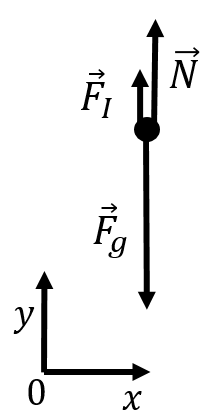
\includegraphics[width=0.2\linewidth]{files/elevator_fbd-02a9d537db0b0d02f41808025e78d38d.png}
\caption[]{Free-body diagram for the forces exerted on a person as modelled in a frame of reference that is accelerating downwards.}
\label{fig:newtonslaws:elevator_fbd}
\end{figure}

All of the forces are in the vertical direction, so we only need to write out the $y$ component of Newton's Second Law, which we can easily solve for the normal force:
\begin{equation}
\sum F_y = N+F_I-F_g &=0\\
N + ma -mg &=0\\
\therefore N=m(g-a)
\end{equation}
Remember that you need to be careful about the signs. We have included the fact that $F_I$ is exerted upwards with the plus sign in the first equation (the $y$ component of $\vec F_I=0\hat x+F_I\hat y$ is $+F_I$). We then used the fact that the magnitude of the inertial force is given by $F_I=ma$ in the second line.

You can easily verify that you would obtain the same result in the inertial frame of reference of the ground, where there is no inertial force, but the acceleration is non-zero (and in the negative $y$ direction if we use the same coordinate system):
\begin{equation}
\sum F_y =N-mg = -ma \quad\quad\text{(ground frame of reference)}
\end{equation}
The normal force, which corresponds to weight as read by the scale, is thus $N=m(g -a)$. We should ask ourselves if the result makes sense:

\begin{itemize}
\item Since the dimension of $a$ and $g$ are the same, $m(g -a)$ has the correct dimension of force.
\item If the acceleration, $a$, is zero, then the magnitude is $N=mg$, as it should be if the elevator is at rest with respect to the ground.
\item If the acceleration $a$ is equal to $g$, the normal force exerted by the scale is exactly zero, and your measured weight is zero. This is what we call being ``weightless'', which is not a good description, since the force of weight is still applied, and it is the normal force which is zero.
\item If the acceleration, $a$, is bigger than $g$, then the normal force would be negative. This corresponds to the elevator accelerating downwards faster than gravity, and the model breaks down, since in this case, you would first hit the ceiling of the elevator, which would then exert a downwards normal force with magnitude $m(a+g)$.
\end{itemize}
\end{framed}
\end{framed}

\subsubsection{Summary}

Newton's Three Laws are a theory of classical physics that allow the motion of an object to be fully described by introducing the concepts of force and mass.

Newton's First Law states that objects will not accelerate if no net force is exerted on the object. In particular, this allows inertial frames of reference to be defined as those frames of reference where Newton's First Law holds true.

Newton's Second Law connects dynamics and kinematics by relating the net force exerted on an object (i.e. the vector sum of the forces exerted on an object) to its acceleration and its mass:
\begin{equation}
\vec F^{net} = \sum_i \vec F_i = m\vec a
\end{equation}
Newton's Third law states that forces always come in pairs that are exerted on different objects. If object A exerts a force on object B, then object B exerts a force that is equal in magnitude but opposite in direction on object A.

A force is a mathematical tool introduced in Newton's theory to model how different objects can influence each other. Mass can be thought of as a quantity of matter and is an intrinsic property of an object. Inertial mass refers to how that quantity of matter resists acceleration, whereas gravitational mass refers to how that quantity of mass experiences the force of gravity. As far as we can tell, inertial and gravitational mass are the same.

When applying Newton's theory, the most important part is to identify the forces that act on one object. This can be represented graphically by using a free-body diagram. The following is a common list of forces to consider when identifying the forces exerted on an object:

\begin{itemize}
\item Weight (is the object near the surface of a planet?).
\item Normal forces (is the object in contact with any surface? There could be more than one!).
\item Frictional forces (are there static or kinetic friction forces associated with the normal forces?).
\item Tension forces (is something like a rope pulling on the object?).
\item Drag forces (is the object moving through a fluid?).
\item Spring forces (is there a spring pushing or pulling on the object?).
\item Applied forces (is anything else pushing or pulling on the object?).
\end{itemize}

When applying Newton's Second Law, one needs to choose a coordinate system so that Newton's Second Law can be written out for each component. It is usually good to choose the coordinate system such that the $x$ axis is parallel to the acceleration vector of the object.

When using Newton's Laws to model the motion of an object of mass $m$ in a non-inertial frame of reference that is accelerating with acceleration $\vec a$ relative to an inertial frame of reference, an additional inertial force, $\vec F_I= -m\vec a$, must be included on the object.

\begin{framed}
\textbf{Important Equations}\\
Newton's Second Law, in vector form, can be written as:
\begin{equation}
\sum \vec F = m\vec a
\end{equation}
which is just a short-hand notation for the scalar equations written out for each component:
\begin{equation}
\sum F_x &= ma_x \\
\sum F_y &= ma_y \\
\sum F_z &= ma_z
\end{equation}

The force of gravity (or weight), $\vec F_g$, near the surface of the Earth is given by:
\begin{equation}
\vec F_g = m\vec g
\end{equation}
where Earth's gravitational field has a magnitude of $g=9.8 {\rm N/kg}$.

The force of kinetic friction exerted by one surface on another is given by::
\begin{equation}
f_k=\mu_kN
\end{equation}
where $N$ is the normal force between the two surfaces and $\mu_k$ is the coefficient of kinetic friction. The force of kinetic friction on an object is in the opposite direction from its motion.

The maximum value of the magnitude of the force of static friction between two surfaces with a coefficient of static friction $\mu_s$ between them, can be written as:
\begin{equation}
f_s\leq\mu_sN
\end{equation}
The force of static friction is exerted in the direction opposite of the impeding motion.

Hookes' Law for the force exerted by a spring, is given by the following vector equation:
\begin{equation}
\vec F = -kx \hat x
\end{equation}
where $x$ is the distance by which the spring is compressed or extended relative to its rest length.
\end{framed}

\begin{framed}
\textbf{Important Definitions}\\
\begin{itemize}
\item \textbf{Mass:} A property of matter which describes its resistance to acceleration. SI units: ${\rm \left[{kg}\right]}$. Common variable(s): $M$, $m$.
\item \textbf{Force:} A mathematical object used to describe the interactions of an object with its environment. SI units: ${\rm \left[{N}\right]}$. Common variable(s): $\vec F$.
\item \textbf{Spring constant:} A value which describes the stiffness of a spring, when the restoring force of the spring is modelled using Hooke's Law. SI units: ${\rm \left[{Nm^{ -1}}\right]}$. Common variable(s): $k$.
\item \textbf{Gravitational field:} The strength of the gravitational force per unit mass at a particular location. Under the equivalence principle, this is numerically equal to the acceleration of free-falling object. SI units: ${\rm \left[N/kg (field), ms^{ -2} (acceleration)\right]}$. Common variable(s): $\vec g$.
\item \textbf{Coefficient of friction:} A constant used to determine the magnitude (or the maximal magnitude in the case of static friction) of a friction force between two surfaces based on the normal force exerted perpendicular to those two surfaces. SI units: none. Common variable(s): $\mu$.
\end{itemize}
\end{framed}

\subsubsection{Thinking about the material}

\begin{framed}
\textbf{Reflect and research}\\
\begin{itemize}
\item What was the name of the publication in which Newton's published his three laws, and when was it published?
\item When did Galileo come up with his principle of inertia?
\item Suppose that Newton grew up in an accelerating train, with no knowledge that he is living in an accelerating train. What would Newton's first law look like in this world?
\item When you skate on ice, there is kinetic friction between your skates and the ice. Does the coefficient of kinetic friction depend on the temperature of the ice? If yes, what is the optimal temperature for skating with the least amount of friction?
\end{itemize}
\end{framed}

\begin{framed}
\textbf{To try at home}\\
\begin{itemize}
\item Place two books stacked on each other on the palm of one hand held horizontally. Use your other hand to press down (and forward) on the top book and try to move the bottom book. No matter how hard you push down (to increase the force of friction between the two books), you cannot make the bottom one move. How come?
\end{itemize}
\end{framed}

\begin{framed}
\textbf{To try in the lab}\\
\begin{itemize}
\item Propose an experiment to determine whether gravitational and inertial mass are equal.
\item Propose an experiment to measure the coefficients of static and kinetic friction between a block and a surface.
\end{itemize}
\end{framed}

\subsubsection{Sample problems and solutions}

\paragraph{Problems}

\begin{framed}
\textbf{Problem 5.1}\\
\begin{figure}[!htbp]
\centering
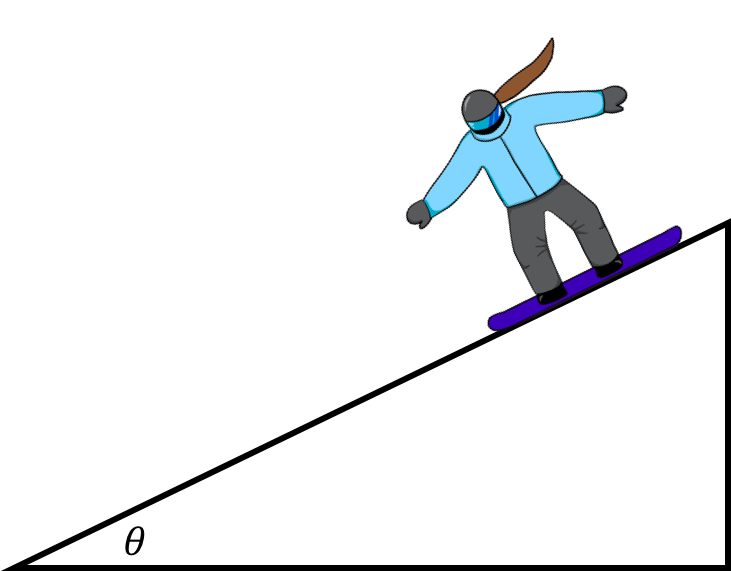
\includegraphics[width=0.4\linewidth]{files/katiesnowboarding-aeca3e46b4630a1e2a156f4b7c0ef841.png}
\caption[]{Katie snowboarding down an incline.}
\label{fig:newtonslaws:katiesnowboarding}
\end{figure}

Katie, an amateur snowboarder, rests at the top of hill inclined by an angle of $\theta =50 {\rm \degree}$ with respect to the horizontal, as shown in Figure~\ref{fig:newtonslaws:katiesnowboarding}. She gracefully slides down the hill until she face-plants into a large pile of snow at the bottom, $40 {\rm m}$ from where she started. If the coefficient of kinetic friction between Katie's snowboard and the hill is $\mu_k=0.45$, how long elapses between when she starts to glide and when she face plants?
\end{framed}

\begin{framed}
\textbf{Problem 5.2}\\
\begin{figure}[!htbp]
\centering
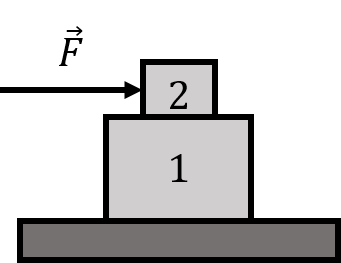
\includegraphics[width=0.2\linewidth]{files/twoboxes-82f598e4aff4cedbd966b3a0553e7309.png}
\caption[]{Two stacked boxes.}
\label{fig:newtonslaws:twoboxes}
\end{figure}

Two boxes with masses, $m_1$ and $m_2$, respectively, are placed on top of one another, as shown in Figure~\ref{fig:newtonslaws:twoboxes}. The coefficient of static friction between the two boxes and between the boxes and the ground is $\mu_s=0.3$. A constant force, $\vec F$, is exerted on box 2, as shown. Show that it is impossible for box 1 to accelerate.
\end{framed}

\paragraph{Solutions}

\begin{framed}
\textbf{Solution 5.1}\\
Before trying to solve the problem, we should think of the strategy that will allow us to model the time that it takes to arrive at the bottom. We know that Newton's Second Law relates the forces on Katie to her acceleration. If we build a model of the forces on Katie, we can then determine her acceleration. Once we know her acceleration, we can use kinematics to determine how long it takes for her to cover the distance of $40 {\rm m}$.

The forces exerted on Katie are:

\begin{enumerate}
\item $\vec F_g$, her weight.
\item $\vec N$, a normal force exerted by the slope.
\item $\vec f_k$, a force of kinetic friction exerted by the slope, with magnitude $f_k=\mu_kN$
\end{enumerate}

This allows us to build a free-body diagram for the forces on Katie, as shown in Figure~\ref{fig:newtonslaws:katieforces}. Since Katie will glide down the slope, her acceleration will be parallel to the slope and downwards, which we showed with a thicker arrow on the free-body diagram. Our free-body diagram also shows the coordinate system that we chose, with the $x$ axis pointing parallel to the acceleration.

\begin{figure}[!htbp]
\centering
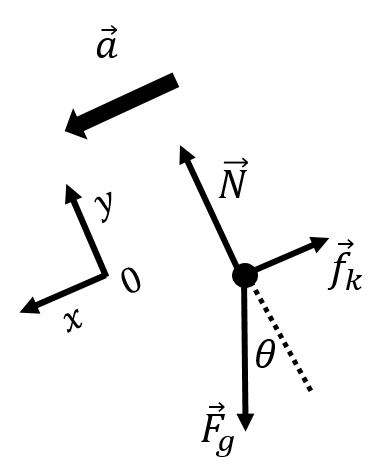
\includegraphics[width=0.3\linewidth]{files/katieforces-8b272d7a912e0bb4ebfc52a709318c4d.png}
\caption[]{Forces acting on Katie as she snowboards.}
\label{fig:newtonslaws:katieforces}
\end{figure}

With a free-body diagram, we can write the $x$ and $y$ components of Newton's Second Law. In the $x$ direction, both the force of friction and the weight have components. The force of friction is in the negative $x$ direction, whereas the component of gravity in the $x$ direction is $F_g\sin\theta$. The acceleration vector is also in the $x$ direction. Putting this altogether into Newton's Second Law:
\begin{equation}
\sum F_x = F_g\sin\theta - f_k &= ma\\
\therefore mg\sin\theta -\mu_k N &= ma
\end{equation}
where we used the fact that the weight is given by $mg$ ($m$ is Katie's mass) and the magnitude of the force of friction is given by $f_k=\mu_kN$.

Next, we write out the $y$ component of Newton's Second Law. The normal force is in the positive $y$ direction, whereas the component of gravity in the $y$ direction is $-F_g\cos\theta$. The acceleration has no component in the $y$ direction. Putting this into Newton's Second Law:
\begin{equation}
\sum F_y = N-F_g\cos\theta &=0\\
\therefore N-mg\cos\theta &=0
\end{equation}

We now have two equations that describe Katie's motion:
\begin{equation}
mg\sin\theta -\mu_k N &= ma\\
N-mg\cos\theta &=0
\end{equation}
We have three unknowns, $m$, $N$, and $a$, but only two equations! Hopefully, one of these will cancel out! At this point, all of the physics for the problem is done! We can now proceed to solve these equations to find the acceleration. The second equation allows us to solve for the normal force, $N=mg\cos\theta$, which we substitute into the first equation:
\begin{equation}
mg\sin\theta -\mu_k N &= ma\\
\therefore mg\sin\theta -\mu_k mg\cos\theta &= ma\\
\end{equation}
As you can see, the mass $m$ can be cancelled out of this equation, and we can find the acceleration:
\begin{equation}
a&=g\sin\theta -\mu_k g\cos\theta\\
&=g(\sin\theta-\mu_k\cos\theta)\\
&=(9.8 {\rm N/kg})\left(\sin(50 {\rm \degree})-(0.45)\cos(50 {\rm \degree})\right)\\
&=4.67 {\rm N/kg}
\end{equation}
At this point, we should ask ourselves if our result makes sense. In particular, we have found that the acceleration has unit of ${\rm N/kg}$ instead of ${\rm m/s^2}$. A quick examination of Newton's Second Law shows us that these two units are equivalent:
\begin{equation}
F &= ma\\
a &= \frac{F}{m}\\
\therefore {\rm [a]} &= \frac{\rm [F]}{\rm [m]}=\frac{\rm N}{\rm kg}
\end{equation}
Often, one write the magnitude of the Earth's gravitation field as $g=9.8 {\rm m/s^2}$, since it has the same dimension as acceleration, and does indeed correspond to the acceleration that is felt by falling objects near the surface of the Earth. In fact, $g$, is usually defined as the acceleration of object near the Earth, although this is misleading, as it requires that inertial and gravitational mass be the same.

Knowing that Katie's initial velocity is $v_{0x}=0 {\rm m/s}$, her acceleration is $a_x=a=4.67 {\rm m/s^2}$ in the $x$ direction (the same direction as the slope), and the distance that she must travel is $x=40 {\rm m}$, we can find the time it takes for her to face-plant. If we set the origin of the $x$ axis where she starts (so that her initial position along the $x$ axis, $x_0=0$), the distance that she covered in the time, $t$, is given by:
\begin{equation}
x(t)&=x_0+v_{0x}t+\frac{1}{2}at^2\\
40 {\rm m}&=(0)+(0)t+\frac{1}{2}(4.67 {\rm m/s^2})t^2\\
\therefore t&=\sqrt{\frac{2(40 {\rm m})}{(4.67 {\rm m/s^2})}}=4.14 {\rm s}
\end{equation}
Katie has $4.14 {\rm s}$ of gliding bliss before face-planting into the large pile of snow.
\end{framed}

\begin{framed}
\textbf{Solution 5.2}\\
The only way for box 1 to accelerate is if box 2 ``drags'' box 1 along with it through a force of friction exerted at the interface between box 1 and box 2. We need to show that the force of (static) friction exerted by the ground on box 1 will always be at least as large as the force of friction exerted by box 2 on box 1. The largest force of friction that box 2 can exert on box 1 is a force of static friction, so we model all forces between surfaces as forces of static friction.

The forces on box 2 are:

\begin{itemize}
\item $\vec F_{2g}$, its weight.
\item $\vec N_2$, a normal exerted by box 1.
\item $\vec f_{2s}$, a force of static friction exerted by box 1.
\item $\vec F$, the applied force.
\end{itemize}

The forces on box 1 are:

\begin{itemize}
\item $\vec F_{1g}$, its weight.
\item $-\vec N_2$, a normal force exerted by box 2 (downwards).
\item $-\vec f_{2s}$, a force of static friction exerted by box 2.
\item $\vec N_1$, a normal force exerted by the ground.
\item $\vec f_{1s}$, a force of static friction exerted by the ground.
\end{itemize}

The are illustrated in the free-body diagram in Figure~\ref{fig:newtonslaws:twoboxes_fbd}

\begin{figure}[!htbp]
\centering
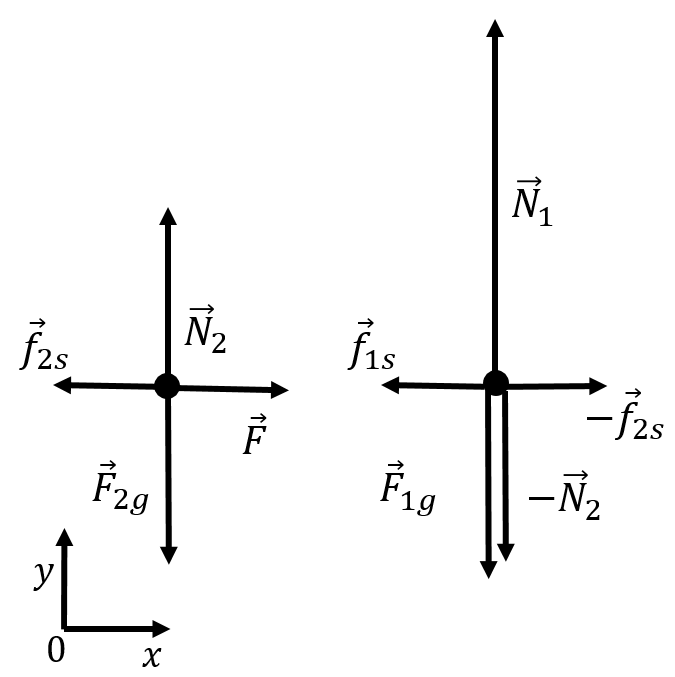
\includegraphics[width=0.4\linewidth]{files/twoboxes_fbd-dc08f10420c8f2ae6d0e00a989fceb10.png}
\caption[]{Forces on the two boxes.}
\label{fig:newtonslaws:twoboxes_fbd}
\end{figure}

Considering the $y$ component of Newton's Second Law for box 2 (the top box), we can find the value of the normal force exerted by box 1:
\begin{equation}
\sum F_y &= N_2 - F_{2g} = 0\\
\therefore N_2 &= m_2 g
\end{equation}
The maximal magnitude of the force of static friction, $f_{2s}$, between the two boxes is given by:
\begin{equation}
f_{2s} = \mu_sN_2 = \mu_s m_2g
\end{equation}
This is the maximal magnitude of the force that can accelerate box 1. Considering the $y$ component of Newton's Second Law applied to box 1, we can find $N_1$, the normal force exerted by the ground:
\begin{equation}
\sum F_y = N_1 - F_{1g} - N_2 = 0\\
\therefore N_1 = F_{1g}+N_2 = (m_1+m_2)g
\end{equation}
The force of static friction exerted by the ground on box 1 will be in the opposite direction as the force of static friction exerted by box 2. The maximal magnitude of the force of static friction exerted by the ground is given by:
\begin{equation}
f_{1s} = \mu_sN_1 = \mu_s (m_1+m_2)g
\end{equation}
We can see that the maximal force of static friction exerted by the ground will always exceed the magnitude of the force of static friction exerted by box 2. It is thus impossible to push on box 2 to make box 1 move (as long as the force of static friction between the two boxes and the box and the ground are the same).
\end{framed}